\documentclass{article}
\usepackage{amsmath}
\usepackage{tikz}
\usepackage[a4paper]{geometry}
\usepackage{fancyhdr}
\pagestyle{fancy}
\lhead{Funktionsscharen}
\rhead{April 2025}
\begin{document}
 
\section{Funktionsscharen}
 
\begin{minipage}[t]{\dimexpr\textwidth-5cm}
 Eine Funktionsschar ist eine Funktion, welche von einem oder mehreren weiteren Parametern abhängig ist. Eine Funktion namens $f$ welche zudem vom Parameter $a$ abhängig ist folgt der Form
 \[
  f_a(x) = \textellipsis
 \]
 
\subsection{Berechnen}
 Funktionsscharen können, genau so wie normale Funktionen auch, mit anderen Werten gleichgesetzt werden um den Wert bestimmter Variablen oder Parameter zu bestimmen.
\vspace{0.4em}
 
\end{minipage}
\hfill
\begin{minipage}[t]{5cm}
  \centering
  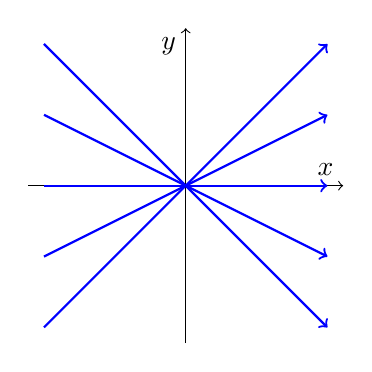
\begin{tikzpicture}[baseline=(current bounding box.north)]
  \draw[->] (-2,0) -- (2,0) node[above left] {$x$};
  \draw[->] (0,-2) -- (0,2) node[below left] {$y$};
   
  \draw[->, blue, thick] (-1.8,-1.8) -- (1.8,1.8);   
  \draw[->, blue, thick] (-1.8,-0.9) -- (1.8,0.9);   
  \draw[->, blue, thick] (-1.8,0) -- (1.8,0);   
  \draw[->, blue, thick] (-1.8,0.9) -- (1.8,-0.9);   
  \draw[->, blue, thick] (-1.8,1.8) -- (1.8,-1.8); 
\end{tikzpicture}
\end{minipage}
Wird nach einer Stelle, wie der Nullstelle, Extremstelle, etc, einer Funktionsschar aufgelöst, ist davon auszugehen, dass das $x$ in Abhängigkeit von dem Parameter liegt.   
Beim Ableiten wird der Parameter wie eine Konstante behandelt. 
 
\subsection{Ortskurven}
Die Kurve, welche durch alle besondere Punkte, wie z.B. alle Nullstellen, Extremstellen oder Wendepunkte, einer Funktionsschar geht, ist eine Ortskurve dieser.
 
\begin{enumerate}
 \item Bestimmen der $x$-Koordinate einer besonderen Stelle in Abhängigkeit vom Parameter. Dies geschieht so wie bei normalen Funktionen, nur das als Ergebnis keine Zahl sondern eine Gleichung für die $x$-Koordinate des Punktes, $p_x$, in abhängig von $a$ ist.
\end{enumerate}   
\begin{minipage}[t]{\dimexpr\textwidth-5cm}
 \begin{enumerate} 
 \item[2.] Bestimmen der dazugehörigen $y$-Koordinate. Dafür muss der $y$-Wert der Funktionsschar bei der besonderen Stelle gefunden werden, heißt dass das bestimmte $p_x$ als $x$ in die Funktionsschar einsetzen werden muss. Somit ist jeder Punkt von $(p_x \,|\, f_a(p_x))$ auf der Ortskurve. Weil das $x$ durch das $p_x$ ersetzt wurde, welches in Abhängigkeit von $a$ steht, ist $f_a(p_x)$ nun ausschließlich von $a$ abhängig.
 \item[3.] Finden der Ortskurvenfunktion $t(x)$. Es gilt bereits $t(p_x) = f_a(p_x)$ mit $p_x \sim a$, die Ortskurvenfunktion $t(x)$ soll aber nur von $x$ abhängen. Dies kann erreicht werden,
 \end{enumerate}
 \end{minipage}
\hfill
\begin{minipage}[t]{5cm}
  \centering
  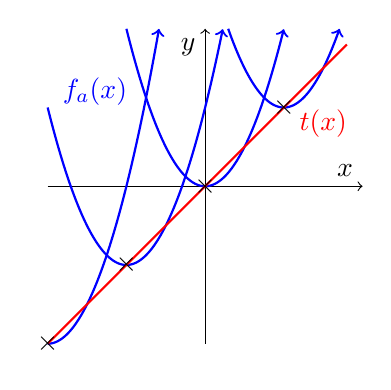
\begin{tikzpicture}[baseline=(current bounding box.north)]
  \draw[->] (-2,0) -- (2,0) node[above left] {$x$};
  \draw[->] (0,-2) -- (0,2) node[below left] {$y$};
  
  \draw[->, blue, thick, domain=-2:-2+sqrt(2*(2+2))/2, samples=100] plot (\x, {2*(\x+(2))^2+(-2)});
  \draw[->, blue, thick, domain=-2:-1+sqrt(2*(2+1))/2, samples=100] plot (\x, {2*(\x+(1))^2+(-1)});
  \draw[->, blue, thick, domain=0-sqrt(2*(2+0))/2:0+sqrt(2*(2+0))/2, samples=100] plot (\x, {2*(\x+(0))^2+(0)});
  \draw[->, blue, thick, domain=1-sqrt(2*(2+-1))/2:1+sqrt(2*(2+-1))/2, samples=100] plot (\x, {2*(\x+(-1))^2+(1)});
 
  \draw[red, thick] (-2,-2) -- (1.8,1.8);
 
  \node[] at (-2,-2) {$\times$};
  \node[] at (-1,-1) {$\times$};
  \node[] at (0,0) {$\times$};
  \node[] at (1,1) {$\times$};
  
  \node[red] at (1.5,0.8) {$t(x)$};
  \node[blue] at (-1.4,1.2) {$f_a(x)$}; 
\end{tikzpicture}
\end{minipage}
\begin{enumerate}
 \vspace{-0.7em} 
 \item[] indem ein $a \sim x$ gefunden und eingesetzt wird. Gefunden werden kann dieses, indem $x = p_x$ nach $a$ aufgelöst wird. Dieses $a$ kann in das bereits bestimmte $t(p_x) = f_a(p_x)$ eingesetzt werden, sodass eine von $x$ abhängige Funktion, welche die Ortskurve beschreibt rauskommt. Diese kann als $t(x)$ genutzt werden.
\end{enumerate}
 
\subsection{Beispiel}
Gegeben ist die Funktionsschar $f(x)=x^2+a \cdot x$, zu welcher es gilt die Ortskurve der Minima zu finden. 
\begin{enumerate}
 \item Das Minima ist bei $f'(x)=0$, heißt $2x+a=0 \implies x=-0.5a$. Somit ist die x-Komponente des Punktes $p_x=-0.5a$
 \item Wird das gefundene $p_x$ in das gegebene $f(x)$ eingesetzt, so ist die gesamte Koordinate eines Maxima immer beim Punkt $\left(-0.5a \,\middle|\, \left(-0.5a\right)^2-0.5a \cdot a\right)$
\end{enumerate}
  
\begin{minipage}[t]{\dimexpr\textwidth-5cm} 
 \begin{enumerate} 
 \item[3.] $x = -0.5a \implies a = -2x$, welches in den Punkt eingesetzt $\left(x \,\middle|\, x^2+x \cdot \left(-2x\right)\right)$. Dies kann als Funktion $t(x)=x^2+x \cdot (-2x)$ oder vereinfacht $t(x)=-x^2$ angesehen werden, welche die Ortskurve korrekt beschreibt.
 \end{enumerate}
 Somit verbindet nun $t(x)$ alle Minima der gegebenen Funktion $f(x)$. \newline
 Das auflösen von $p_x \sim a$ gefolgt von $a \sim x$ mag wie ein unnötiger Schritt, welcher übersprungen werden kann, scheinen, ist dies aber nicht. Bei komplexeren Funktionen sind oftmals nach naivem auflösen die $x$-Werte beide Funktionen und des Punktes auf unterschiedlichen skalen.
\end{minipage} 
\hfill 
\begin{minipage}[t]{5cm} 
 \centering
 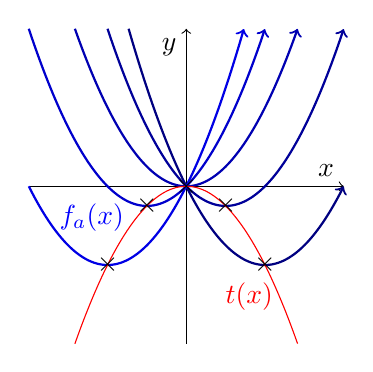
\begin{tikzpicture}[baseline=(current bounding box.north)]
  \draw[->] (-2,0) -- (2,0) node[above left] {$x$};
  \draw[->] (0,-2) -- (0,2) node[below left] {$y$};
  
  \draw[->, blue!50!black, thick, domain=0.5*(-sqrt((-2)^2+8)-(-2)):2, samples=100] plot (\x, {(\x)^2+\x*(-2)});
 \draw[->, blue!60!black, thick, domain=0.5*(-sqrt((-1)^2+8)-(-1)):0.5*(sqrt((-1)^2+8)-(-1)), samples=100] plot (\x, {(\x)^2+\x*(-1)});
 \draw[->, blue!70!black, thick, domain=0.5*(-sqrt((0)^2+8)-(0)):0.5*(sqrt((0)^2+8)-(0)), samples=100] plot (\x, {(\x)^2+\x*(0)});
 \draw[->, blue!80!black, thick, domain=0.5*(-sqrt((1)^2+8)-(1)):0.5*(sqrt((1)^2+8)-(1)), samples=100] plot (\x, {(\x)^2+\x*(1)});
 \draw[->, blue!90!black, thick, domain=-2:0.5*(sqrt((2)^2+8)-(2)), samples=100] plot (\x, {(\x)^2+\x*(2)});
 
 \draw[red, domain=-sqrt(2):sqrt(2), samples=100] plot (\x, {-(\x)^2}); 
  
 \node[red] at (0.8,-1.4) {$t(x)$};
 \node[blue] at (-1.2,-0.4) {$f_a(x)$}; 
  
 \node[] at (-1,-1) {$\times$}; 
 \node[] at (-0.5,-0.25) {$\times$};
 \node[] at (0,0) {$\times$}; 
 \node[] at (0.5,-0.25) {$\times$};
 \node[] at (1,-1) {$\times$}; 
 \end{tikzpicture}
\end{minipage} 
 
 
\end{document} 
 
 
 
 
 
 
 
 
 
